\documentclass[]{article}
\usepackage[spanish.mexico]{babel}
\usepackage[T1]{fontenc}
\usepackage[utf8]{inputenc}
%\usepackage{lmodern}
\usepackage[a4paper]{geometry}

%Graficos e imagenes
\usepackage{graphicx}
%\graphicspath{ Imagenes/ }

\usepackage{cite}

%Grafico de barras
%\usepackage{pgfplots}


\usepackage{tikz}
\usepackage[american voltages, american currents,siunitx]{circuitikz}

%\title{Proyecto de Optimización de Energía}
%\author{Pablo Vivar Colina}
%\date{Mayo 2018}



\begin{document}
	
%\usepackage[top=2cm,bottom=2cm,left=1cm,right=1cm]{geometry}


\begin{titlepage}
     \begin{center}
	
\includegraphics[width=0.09\textwidth]{UNAM}\Large Universidad Nacional Autónoma de México
        	
\includegraphics[width=0.09\textwidth]{FI}\\[1cm]
        \Large Facultad de Ingeniería\\[1cm]
       % \Large División de Ciencias Básicas\\[1cm]
         \Large Laboratorio de Fundamentos de Control(6655)\\[1cm]
         %la clave antes era:4314
         \footnotesize Profesor: Salcedo Ubilla María Leonor Ing.\\[1cm]
        \footnotesize Semestre 2019-1\\[1cm]
        
       

        \Large Práctica No. 1\\[1cm]
        
           

\Large Introdcción MATLAB
        
         %Texto a la derecha
          \begin{flushright}
\footnotesize  Grupo 2\\[0.5cm]
\footnotesize Brigada: 4\\[0.5cm]
\footnotesize Rodrigo Adrián Martínez López\\[0.5cm]
\footnotesize Vivar Colina Pablo\\[0.5cm]
 \end{flushright}
    %Texto a la izquierda
          \begin{flushleft}
        \footnotesize Ciudad Universitaria Agosto de 2018.\\
          \end{flushleft}
         
          
        %\vfill
        %\today
   \end{center}
\end{titlepage}
 %agregar portada

%\maketitle

\tableofcontents  % Write out the Table of Contents

%\listoffigures  % Write out the List of Figures

\section{Resumen}

\section{Introducción}


\subsection{NI ELVIS}

Para crear una aplicación completa de NI ELVIS, explore otras soluciones de laboratorio para NI ELVIS.\\

Proporciona una experiencia de aprendizaje basada en proyectos, usando medidas en línea y diseño práctico y embebido.\\

El NI Educational Laboratory Virtual Instrumentation Suite (NI ELVIS) es un dispositivo modular de laboratorio educativo de ingeniería desarrollado específicamente para la academia. Con este enfoque práctico, los profesores pueden ayudar a los estudiantes a aprender habilidades de ingeniería prácticas y experimentales. NI ELVIS incluye un osciloscopio, multímetro digital, generador de funciones, fuente de alimentación variable, analizador de Bode y otros instrumentos comunes de laboratorio. Puede conectar una PC al NI ELVIS usando USB y desarrollar circuitos en su protoboard desmontable.\cite{NationalInstruments2018}\\


\section{Objetivos}

	\begin{itemize}
			\item Utilizar la herramientas de National Instruments para verificar las ecuaciones de función de transferencia
	\end{itemize}


\section{Materiales y métodos}

	\begin{itemize}
		\item NI Elvis
		\item Computadora con Suite de herramientas Texas Instruments
	\end{itemize}
	
\section{Resultados}



Se usa el circuito operacional con realimentacion negativa.\\

\begin{itemize}
	
	\item 2->Entrada Inversora
	\item 3->Entrada no inversora
	\item 4->Fuente -10[V]
	\item 5->Vacío
	\item 6->Salida
	\item 7->Fuente +10[V]
\end{itemize}

\begin{equation}
  \frac{1.42}{s^2+2.42s+1.42}
\end{equation}

Función de transferencia




%AQUI VAMOS

\begin{figure}[h!]
	\centering
	\begin{circuitikz}
		
		\draw
		
		%Generador de funciones
		
		(-6,0.5) to   (-6,-0.5) node[ground]{}
		(-6,0.5)--(-5,0.5)
		(-5,0.5)to[vco,l=$G$](-4,0.5)
		
		
		%resistencia1
		(-1,0.5)to[R,l=$R_1$](-4,0.5)
				
			%resistencia5
		(-1.75,0.5)--(-1.75,-2.5)
		(-1.75,-2.5)to[R,l=$R_5$](5,-2.5)
		(5,-2.5)--(5,-0.5)
		
	
	    (1,1.5)--(1.5,1.5)
	     (2,1.5) node {$V_S$}
	
		%Resistencia2
		(-1,0.5)--(-1,1.5)
		(-1,1.5)to[R,l=$R_2$](1,1.5)
		(1,1.5)--(1,0)
	
	(0,0) node[op amp] (opamp1) {741}
	%tierra a no invesora
	(-1.25,-0.5)  to  (-1.25,-1) node[ground]{}
	
	%Resistencia 3 
	(1,0)to[R,l=$R_3$](3,0)
	
	%Resistencia4
	(3,0)--(3,1)
	(3,1)to[R,l=$R_4$](5,1)
	(5,1)--(5,-0.5)
	
	(4,-0.5) node[op amp] (opamp1) {741}
		%tierra a no invesora(-1,-3) node {$X_1$}
		(2.75,-1)  to  (2.75,-1.5) node[ground]{}
		
		(5.5,-0.5) node {$V_X$}
		;

	\end{circuitikz}
	\caption{Circuito de Amplificadores operacionales}
	\label{fig:OpAmpCircuito}
\end{figure}

En la figura \ref{fig:OpAmpCircuito} se puede pareciar el circuito que se ocupó en la experimentación.\\

\begin{figure}[h!]
	\centering
	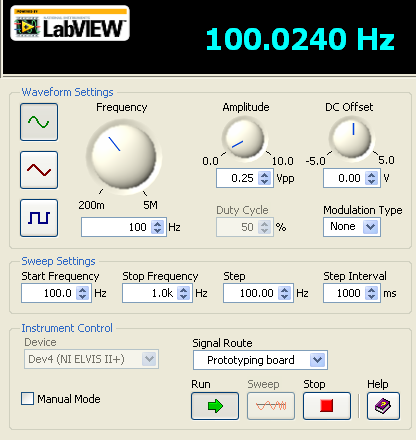
\includegraphics[width=0.6\textwidth]{Imagenes/fgen250mVpp100Hzdosaplisprac4}
	\caption{Generador de funciones}
	\label{fig:primerCircuito}
\end{figure}

En la figura \ref{fig:primerCircuito} se puede apreciar la configuración del generador de funciones el cual genera una señal senoidal de 100 [Hz] y con 0.25 [Vpp].\\

\begin{figure}[h!]
	\centering
	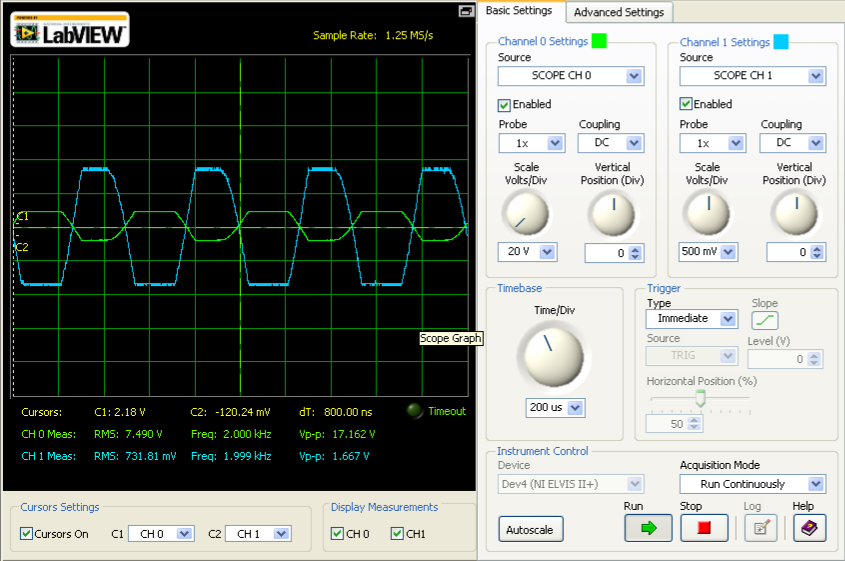
\includegraphics[width=0.6\textwidth]{Imagenes/r5es10kfrec2Kprac4.png}
	\caption{Valor de la resistencia 5 del circuito \ref{fig:OpAmpCircuito} con 10 k, con frecuencia en la señal de 2[kHz]}
	\label{fig:2K}
\end{figure}

En la figura \ref{fig:OpAmpCircuito} se aprecia la respuesta del circuito mostrado anteriormente.\\


\begin{figure}[h!]
	\centering
	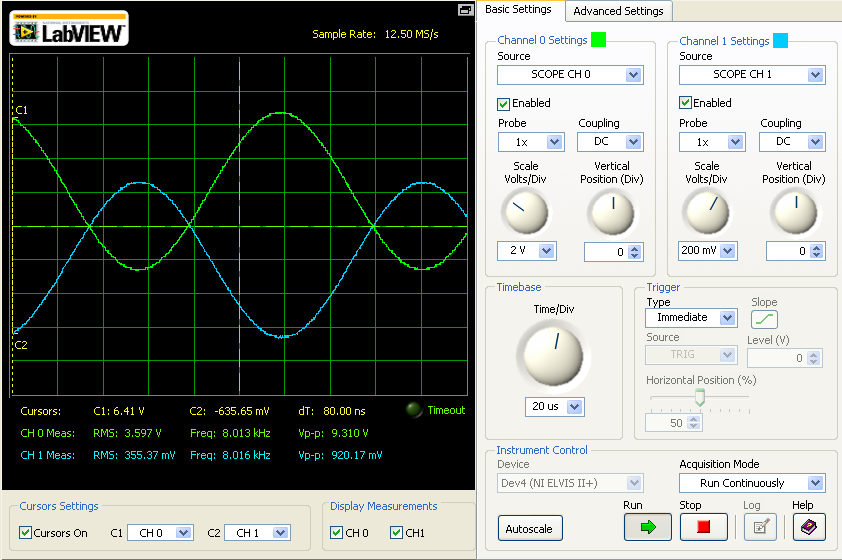
\includegraphics[width=0.6\textwidth]{Imagenes/r5es10kfrecu8Kprac4.png}
	\caption{Valor de la resistencia 5 del circuito \ref{fig:OpAmpCircuito} con 10 k, con frecuencia en la señal de 8[kHz]}
	\label{fig:8K}
\end{figure}

\begin{figure}[h!]
	\centering
	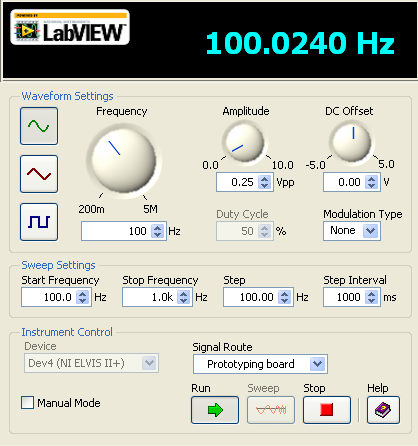
\includegraphics[width=0.6\textwidth]{Imagenes/r5es10kprac4.png}
	\caption{Valor de la resistencia 5 del circuito \ref{fig:OpAmpCircuito} con 10 k}
	\label{fig:noFrec}
\end{figure}

\begin{figure}[h!]
	\centering
	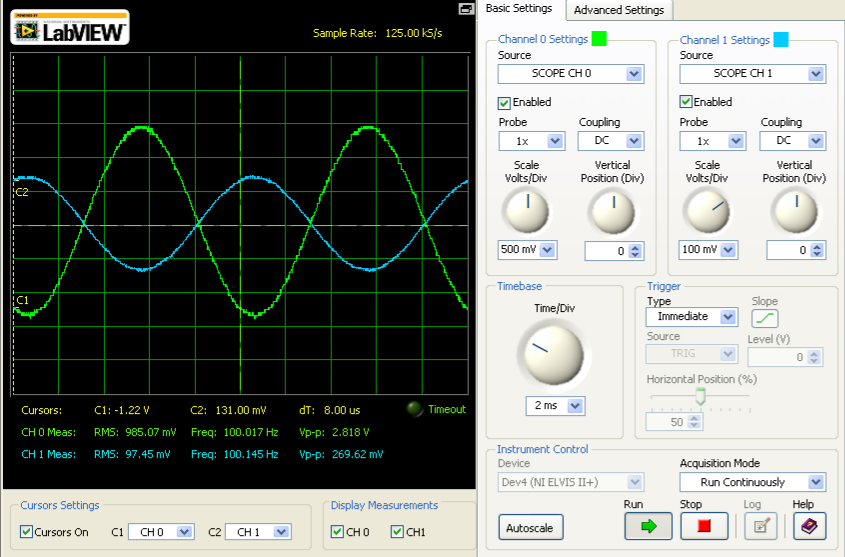
\includegraphics[width=0.6\textwidth]{Imagenes/r5es100kprac4.png}
	\caption{Valor de la resistencia 5 del circuito \ref{fig:OpAmpCircuito} con 100 k}
	\label{fig:100kres}
\end{figure}



\section{Análisis de Resultados}



\section{Conclusiones}


\section{Referencias}

\bibliographystyle{plain}
\bibliography{Referencias.bib}



\end{document}
